\begin{frame}{Installing GNU Octave on MS Windows 10 (1/8)}
\begin{center}
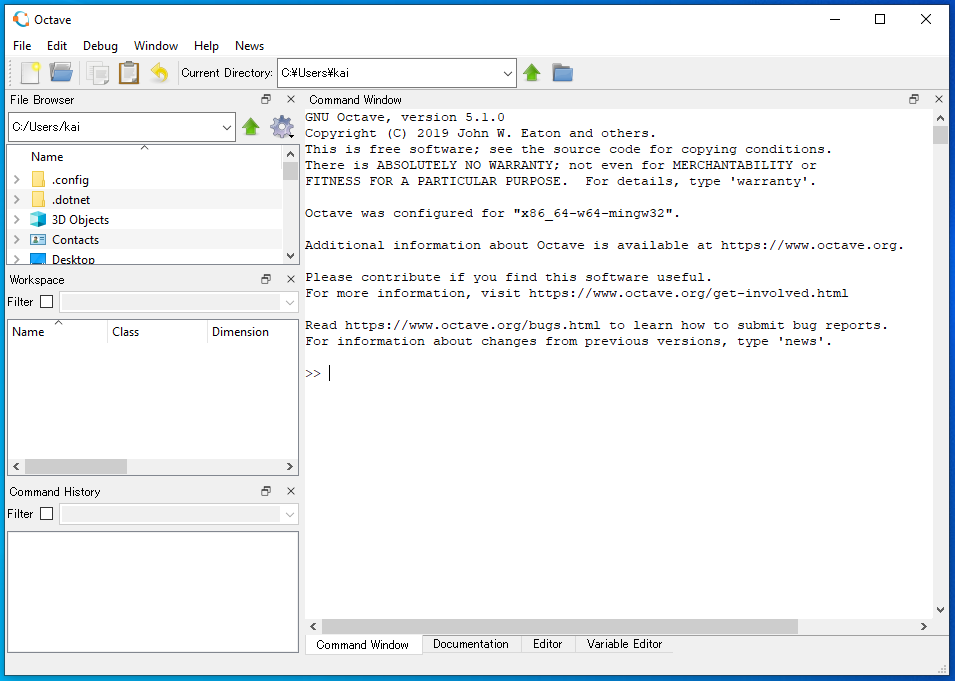
\includegraphics[width=0.8\textwidth]{res/ms_windows/win_octave_gui.png}
\end{center}
\end{frame}



\begin{frame}{Installing GNU Octave on MS Windows 10 (2/8)}
\begin{center}
\url{https://www.octave.org/download}
\end{center}
\begin{columns}
\begin{column}{0.5\textwidth}
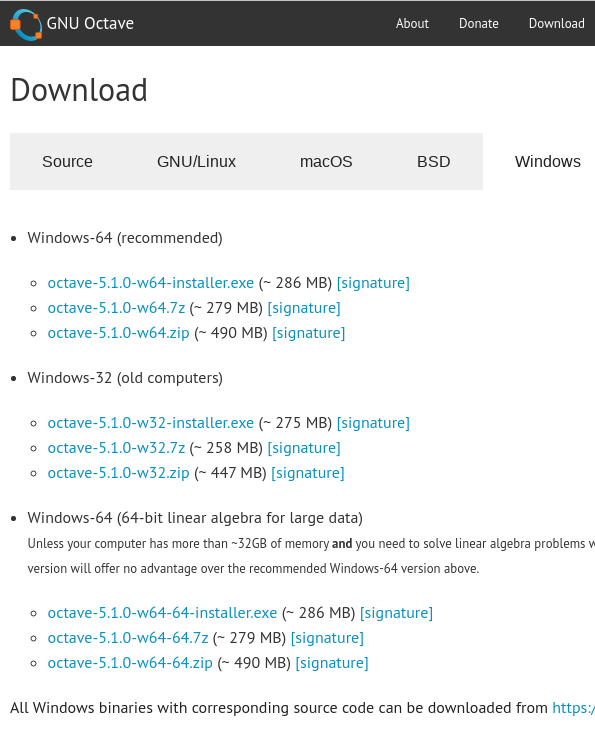
\includegraphics[width=0.9\textwidth]{res/ms_windows/win_download_cropped.png}
\end{column}
\begin{column}{0.4\textwidth}
\begin{itemize}
\itemsep0.8em
\item
\textbf{w32}: 32-bit systems (very old or embedded devices)

\item
\textbf{w64}: 64-bit systems \greencheck

\item
\textbf{w64-64}: 64-bit systems with \textbf{large} main memory
$2^{32} \times 8 \,Bytes = 32 \,GB$\\[0.5em]

Working with dense double matrices with $400,000 \times 100,000$ entries
($\approx 298 \,GB$) \textbf{need} this.
\end{itemize}
\end{column}
\end{columns}
\end{frame}



\begin{frame}{Installing GNU Octave on MS Windows 10 (3/8)}
\begin{columns}
\begin{column}{0.5\textwidth}
\textbf{Ignore} Java warning:
\begin{itemize}
\item
Octave works perfectly without Java.

\item
Octave's Java interface might not work properly.
\end{itemize}

\vspace*{2em}

\textbf{Choose:}
\begin{itemize}
\item
{\color{DarkBlue}OpenBLAS} (usually faster)

{\footnotesize \url{https://www.openblas.net/}}

\item
{\color{DarkBlue}Reference BLAS}

{\footnotesize \url{https://www.netlib.org/blas/}}
\end{itemize}
\end{column}
\begin{column}{0.4\textwidth}
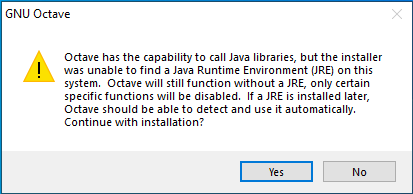
\includegraphics[width=\textwidth]{res/ms_windows/win_install_java_warning.png}
\\[1em]
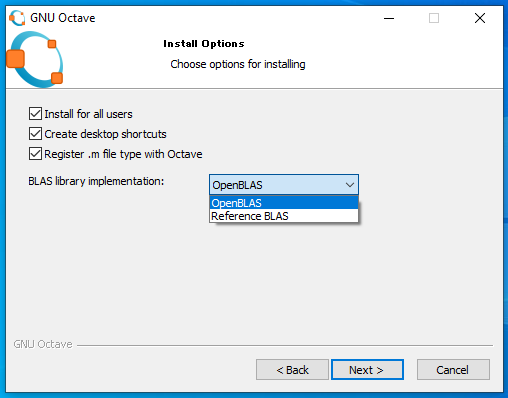
\includegraphics[width=\textwidth]{res/ms_windows/win_install_blas.png}
\end{column}
\end{columns}
\end{frame}



\begin{frame}{Installing GNU Octave on MS Windows 10 (4/8)}
\begin{itemize}
\item
As usual: desktop icons (left) and start menu entries (right).
\end{itemize}
\begin{columns}
\begin{column}{0.4\textwidth}
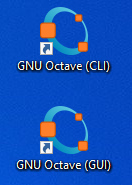
\includegraphics[width=0.6\textwidth]{res/ms_windows/win_install_desktop_icons.png}
\end{column}
\begin{column}{0.4\textwidth}
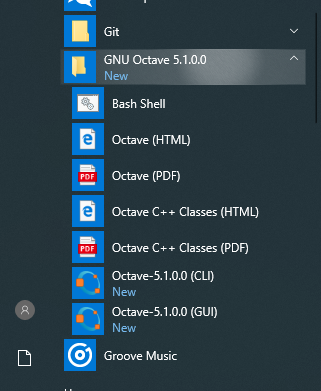
\includegraphics[width=0.8\textwidth]{res/ms_windows/win_install_startmenu_icons.png}
\end{column}
\end{columns}
\begin{itemize}
\item
Start
\begin{itemize}
\item
\textbf{command-line interface (CLI)}
\item
\textbf{graphical user interface (GUI)}
\end{itemize}
\end{itemize}
\end{frame}



\begin{frame}{Installing GNU Octave on MS Windows 10 (5/8)}
\begin{center}
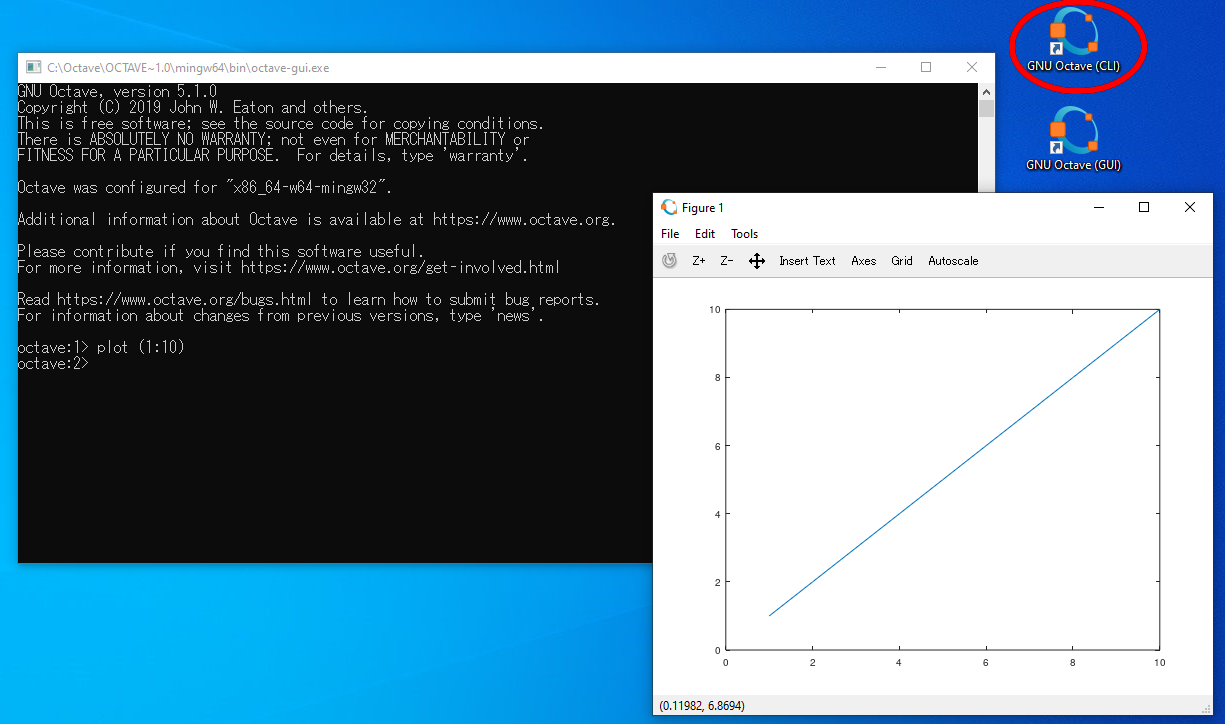
\includegraphics[width=0.9\textwidth]{res/ms_windows/win_octave_cli_plot.png}
\end{center}
\end{frame}



\begin{frame}{Installing GNU Octave on MS Windows 10 (6/8)}
\begin{center}
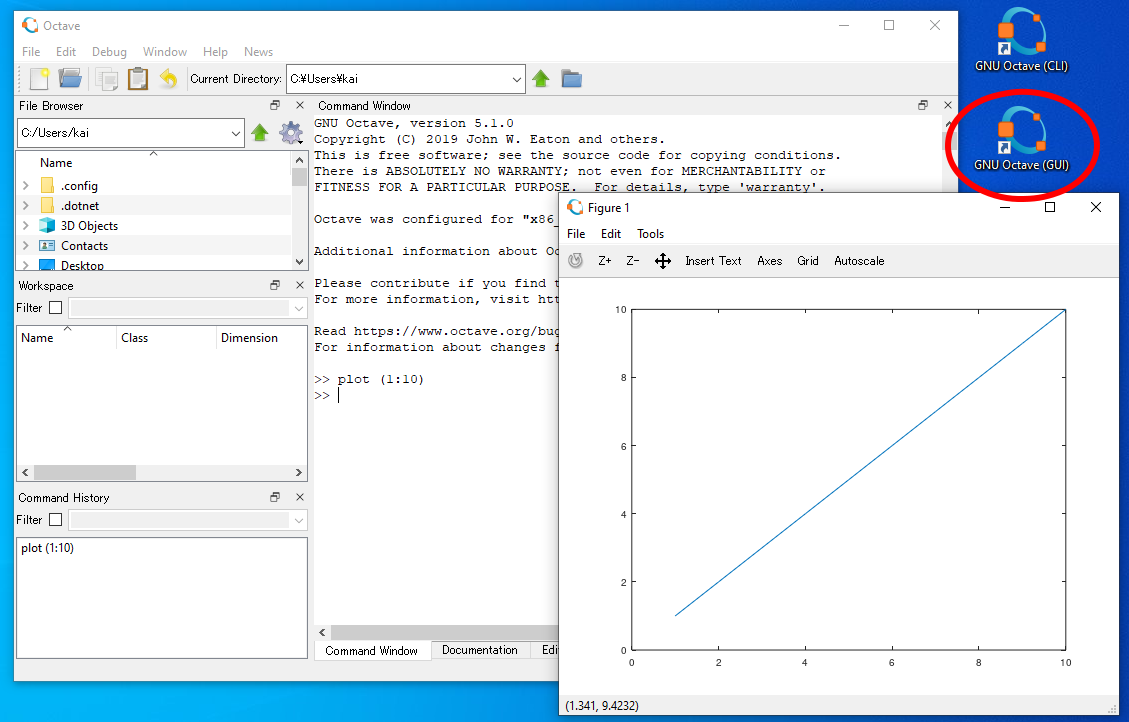
\includegraphics[width=0.9\textwidth]{res/ms_windows/win_octave_gui_plot.png}
\end{center}
\end{frame}



\begin{frame}{Installing GNU Octave on MS Windows 10 (7/8)}
\begin{itemize}
\item
Many \textbf{\color{DarkBlue}Octave Forge} packages precompiled
as part of the installer.
\item
No need to download them, just \textbf{load} them.

$\quad\rightarrow$ \texttt{pkg list}
$\qquad\quad\;\rightarrow$ \texttt{pkg load io}
\end{itemize}
\begin{center}
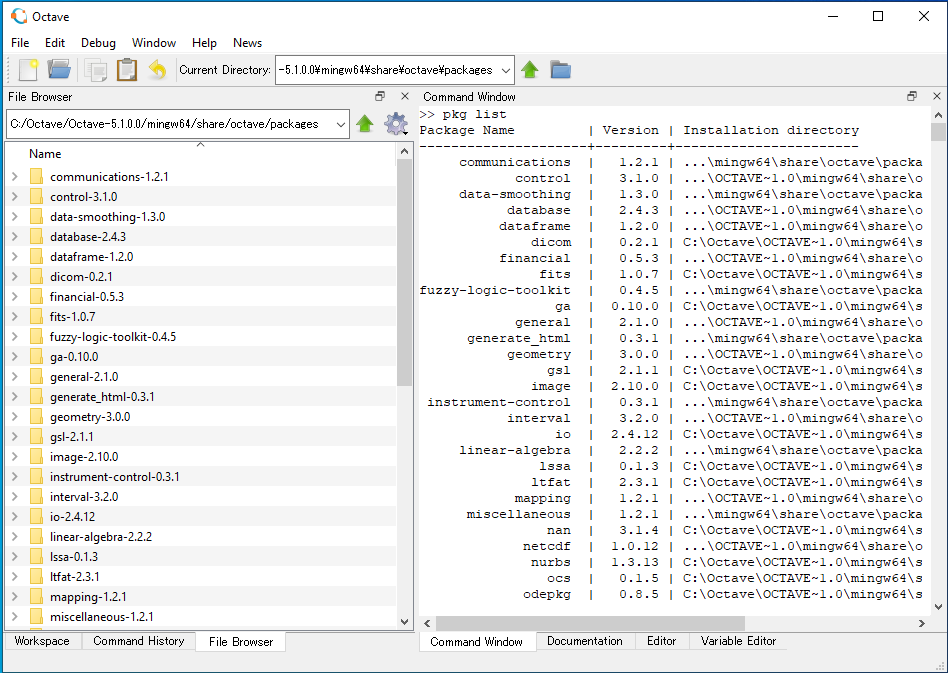
\includegraphics[width=0.6\textwidth]{res/ms_windows/win_octave_packages.png}
\end{center}
\vspace*{-0.8em}
\texttt{C:\textbackslash Octave\textbackslash Octave-5.1.0.0\textbackslash
  mingw64\textbackslash share\textbackslash octave\textbackslash packages}
\end{frame}



\begin{frame}{Installing GNU Octave on MS Windows 10 (8/8)}
\begin{columns}
\begin{column}{0.3\textwidth}
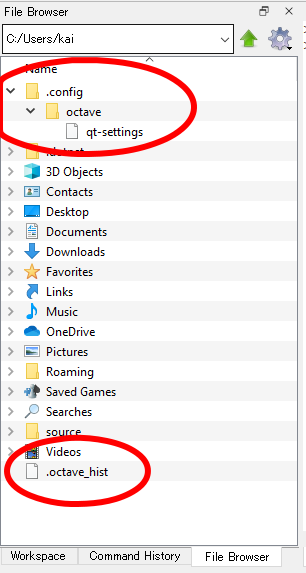
\includegraphics[width=\textwidth]{res/ms_windows/win_octave_settings.png}
\end{column}
\begin{column}{0.6\textwidth}
\begin{itemize}
\itemsep2em
\item
Setting files in User's home directory.

e.g. \texttt{C:\textbackslash Users\textbackslash kai}

\item
Delete them if GUI is not starting.

\item
Use/start Octave without GUI from other programs, see
\texttt{\small C:\textbackslash Octave\textbackslash
Octave-5.1.0.0\textbackslash
octave.vbs}
\end{itemize}
\end{column}
\end{columns}
\end{frame}